\documentclass[8pt,a4paper]{report}
\usepackage{hyperref}
\usepackage[latin1]{inputenc}
\usepackage{xcolor}
\usepackage{textcomp}
\usepackage{amsmath}
\usepackage{amsfonts}
\usepackage{listings}
\usepackage{amssymb}
\usepackage{fancyvrb}
\usepackage{wrapfig}
\usepackage{hyperref}
\usepackage[T1]{fontenc}
\usepackage[scaled]{beramono}
\newcommand\Small{\fontsize{9}{9.2}\selectfont}
\newcommand*\LSTfont{\Small\ttfamily\SetTracking{encoding=*}{-60}\lsstyle}
\usepackage{url}
  \lstset{basicstyle=\ttfamily\tiny\color{blue}}
\usepackage{graphicx}
%\usepackage[]{algorithm2e}
\usepackage{algorithm}
\usepackage{algpseudocode}
\usepackage{pifont}

\title{Project Report\\\textsc{DEVS Ex Machina}}
\author{Ben Cardoen\\Pieter Lauwers\\Stijn Manhaeve\\Tim Tuijn\\Matthijs Van Os}
\date{}
\begin{document}
\maketitle
\tableofcontents{}

%
\chapter{Summary}
%
\section*{}
The project implements a C++ port of the PyPDEVS project, extended with conservative synchronization and a change in system architecture from distributed simulation on several nodes (asymmetric mp) to a symmetric multiprocessing architecture. \\The summarized goal of the project is to provide an implementation of the offered DEVS formalisms with significantly lower execution time by leveraging the smp architecture.

\section*{Terminology}
The literature sometimes exchanges terms, to avoid any confusion the following frequent terms are listed with their associated meaning as used in this document:
\begin{itemize}
  \item Core : alias kernel. Single instance, containing a set of models for which it is responsible, exchanges messages generated by those models and keeps time state. Can correspond with Logical Process in terms of what it represents.
  \item Logical Process : set of models with strong internal coherence.
  \item Distributed parallelism : computation distributed over several physically separated machines communicating by means of a network stack.
  \item SMP : symmetric multiprocessing, running a parallel computation on several distinct CPU cores/threads on the same machine with shared memory (and/or cache).
  \item message : any exchange of high level information between entities, user defined or for inter-kernel synchronization.
  \item lookahead : Timespan relative to current state where the output of the model is not influenced by its input. (as per definition in \cite{cons}, app B)
  \item eot : Earliest output time. Timepoint in future where the core/kernel will output events.
  \item eit : Earliest input time. Timepoint in future where the core/kernel expects to
  be change state on receiving event.
\end{itemize}
Lookahead is collected per model per kernel, eit/eot are based on information from models but determined on a core/kernel level.

\chapter{Architecture Analysis}
\section{Implementation language}
Python is a very powerful language, but due to its interpreted nature it suffers from a performance point of view. Python's GIL \cite{gil} makes this issue even more serious whenever multi-threading is required. Although it relieves the developer from tracking resource allocation, this comes at a price in the overhead caused by the GC. \\
In contrast, C++ offers low-level powerful thread primitives, but requires the developer to have a very deep understanding of parallel programming techniques. By using RAII, a C++ developer can leverage safe resource (de)allocation without losing performance.\\
A significant advantage Python offers a developer is relative cross-platform capability. This is non-trivial for a C++ developer, since at the very least the toolchains will be radically different in usage, and sometimes even in implementation of the C++ standard. The edit-build-test cycle is also non-trivial for a large C++ application, whereas in Python this is negligible. In contrast, Python does not offer the programmer any of the C++ compiler's many compile time checks (static typechecks and program analysis).

\section{Operating system support}
The project requires a compliant C++11 compiler and library, but beyond that is not really bound to special features. For testing, GTest is a requirement, and the only two other dependencies are the ubiquitous Boost and Cereal, the latter is provided with the project as it is header only.

\section{Object representation}
In Python everything is a reference, and since the DEVS formalisms require that the user be allowed to override most of the basic entities, the best representation for an object was a shared\textunderscore ptr. Passing by value could have been safer (e.g. between threads) but would introduce slicing.\\ Another advantage was that we would use as little memory as possible, for example sending a message means passing a const reference to a shared pointer, which is usually equal in size to 2 pointers. By passing by const ref we minimize most of the penalty usually involved in copyconstructing shared pointers. \\
The only downside is the synchronized access to the reference count in the shared pointer. There is also a need for more boilerplate code to use shared pointers in containers (providing pass-through hash function, comparison etc). 

\section{Messaging Size}
A message is constructed once, and after that never copied. Messages are sent and received by reference to smart pointer, incurring a size cost of (on 64-bit platforms) 128bit. The payload (and its size) is irrelevant to the simulation up to the point where the message is actually received. A default implementation allows the payload stored as a std::string, but a specialized message class can be used for sending objects of a different type. When constructing a message by using the functionality provided by the Port class, this happens automatically. When receiving messages, a free function template is provided to extract the object from the message.\\
For example:
\begin{lstlisting}[language=C++,basicstyle=\small\color{black}]
//initialization of necessary objects is left out.
double value;
n_model::t_portptr port;

//create messages that contain a double
auto msgVector = port->createMessages(value);

//say we receive this message somewhere else
n_network::t_msgptr received =  msgVector[0];

//retrieve the data when receiving the message
const double& data = n_network::getMsgPayload<double>(received);

//Assuming that no Z function was applied to the message.
assert(value == data);
\end{lstlisting}
\paragraph{Note} While it is technically possible, we strongly discourage the usage of the following data types in these messages:
\begin{itemize}
	\item raw pointers to heap-allocated object.\\
			Messages can be destroyed during a time warp prior to being delivered to a model. This will result in a memory leak if there are no other references to these objects.
	\item pointers or references to local objects.\\
		When these objects go out of scope, they are destructed, rendering the pointer or reference invalid.
\end{itemize}

\chapter{Design}
\section{Overview}
We've slightly departed from the PyPDEVS structure, to allow for more encapsulation and decoupling of the core entities. This clear separation of data and responsibilities between classes made the threading part of the project easier (no or minimal shared state). See the \hyperref[simpledesign]{Simple Design figure \ref*{simpledesign}}.\\

\begin{figure}[h!]
	\makebox[\textwidth][c]{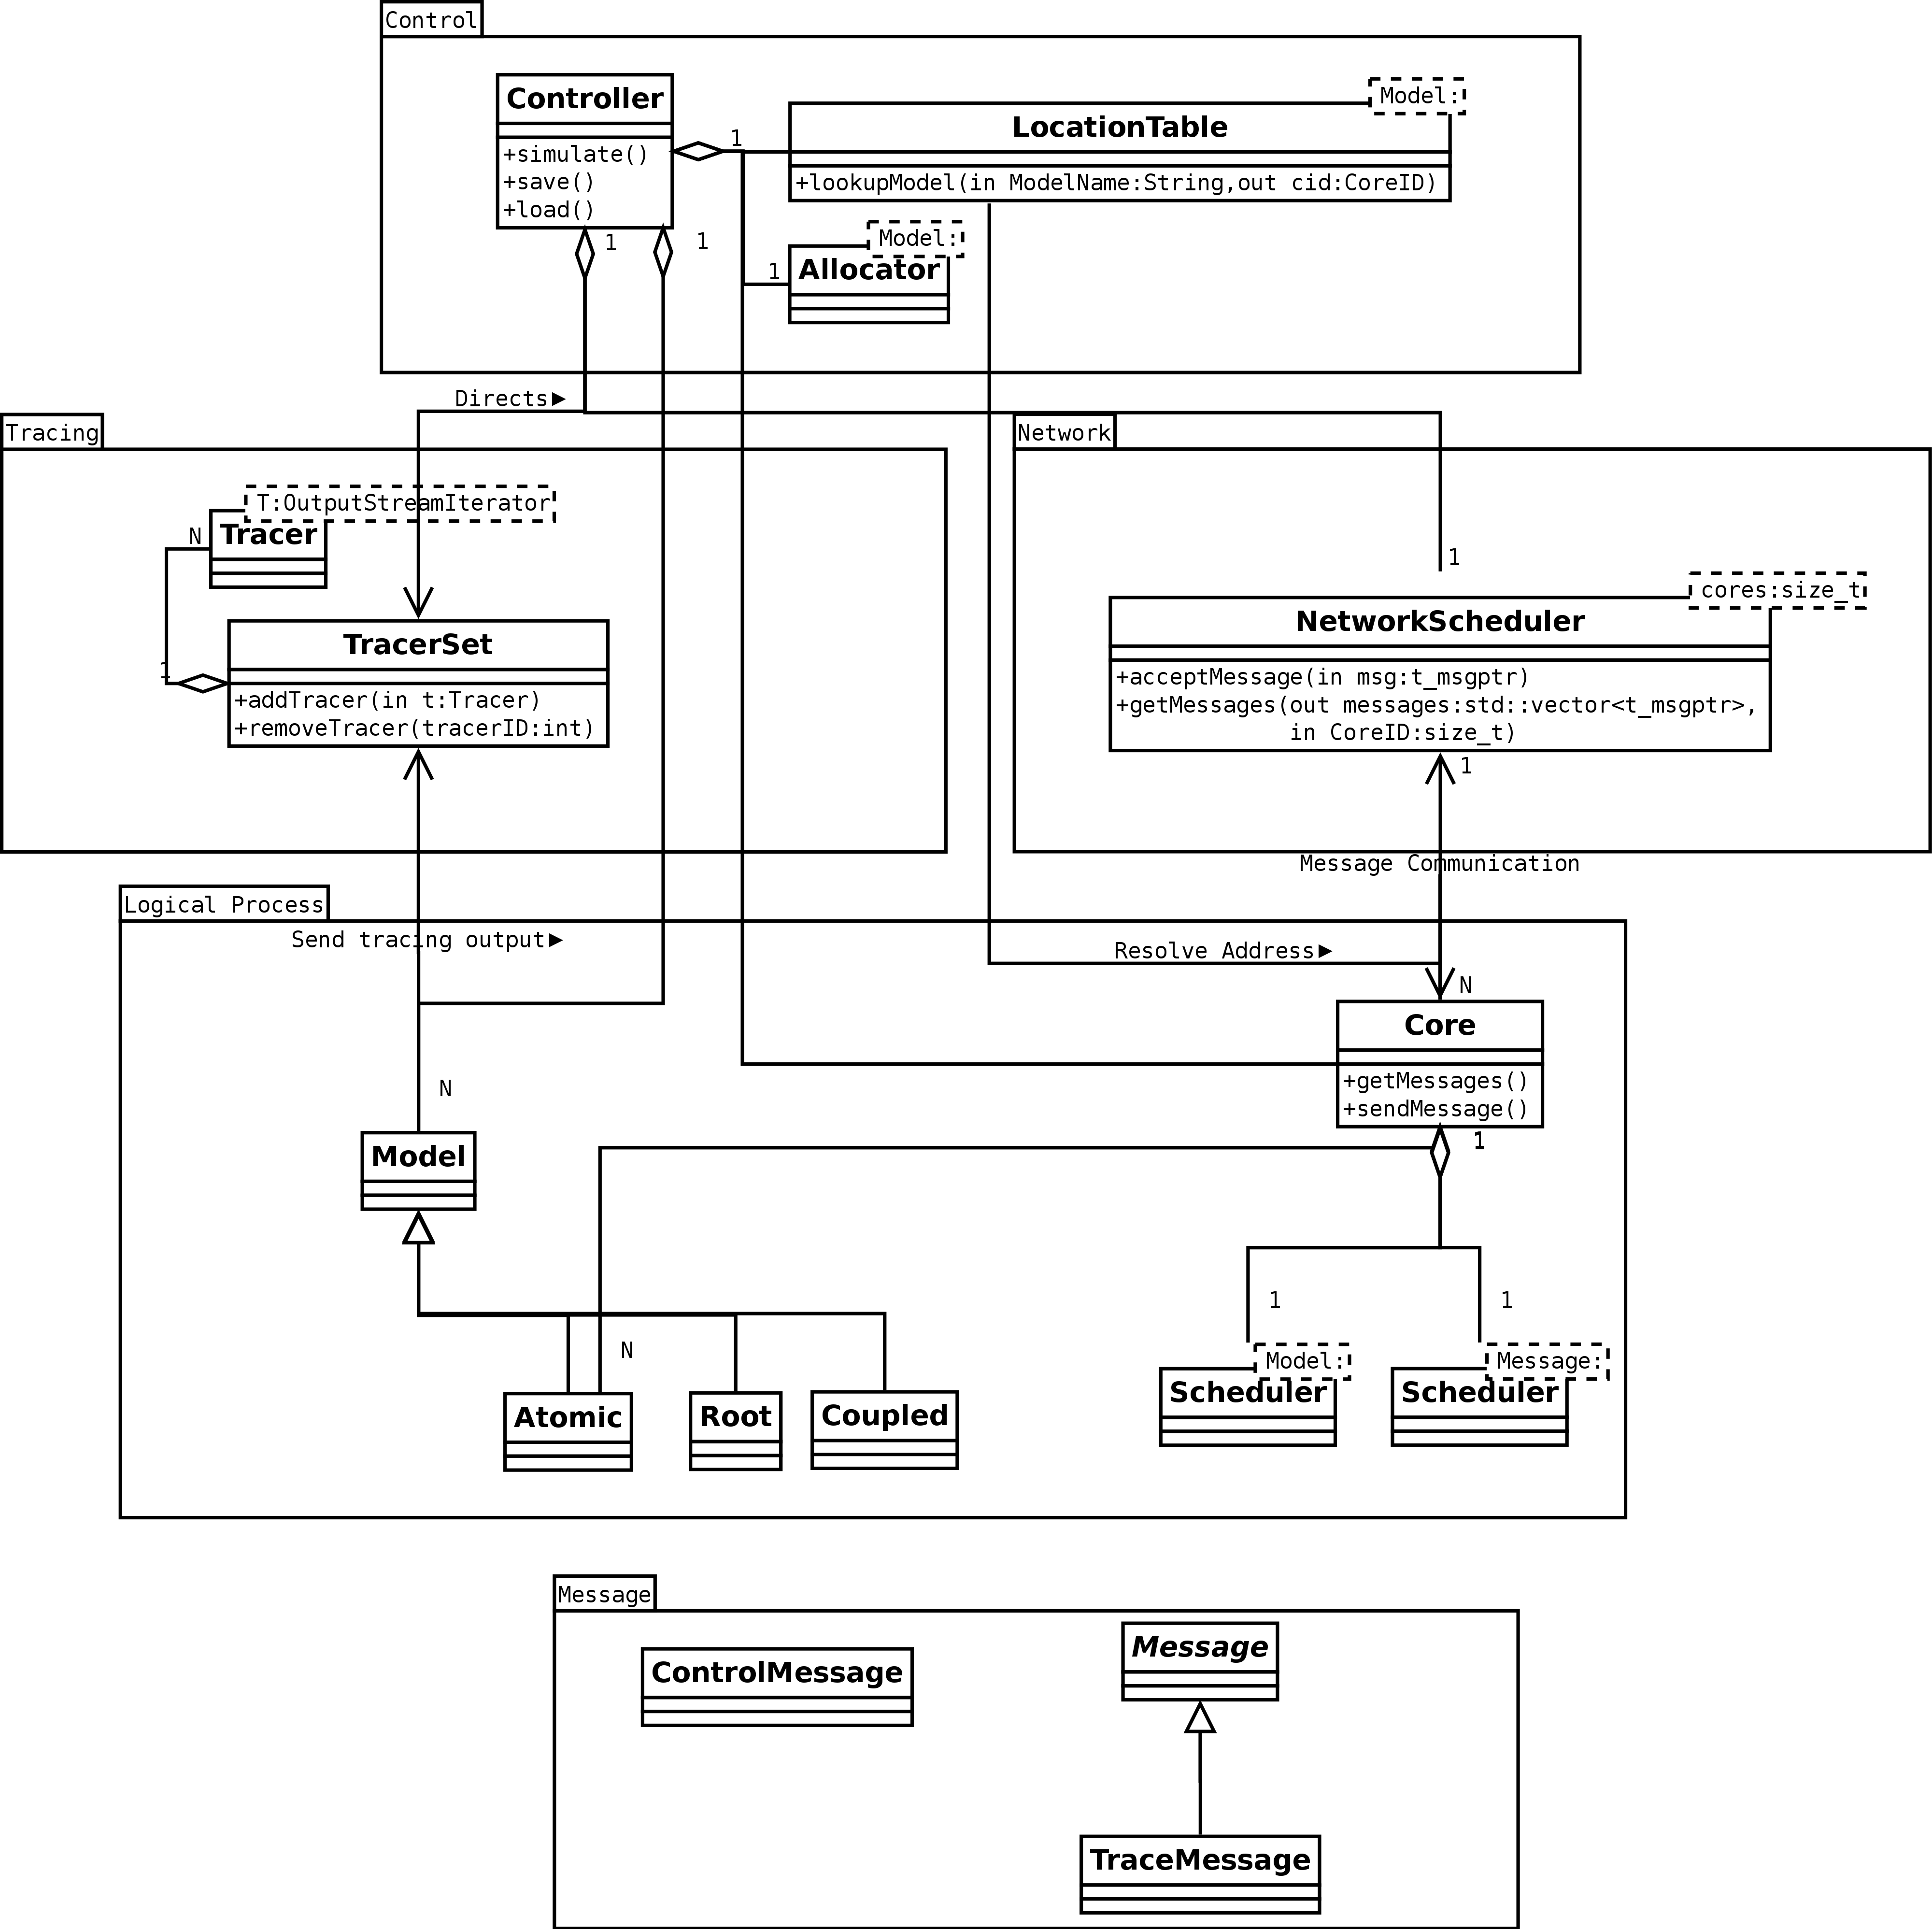
\includegraphics[width=1.5\textwidth]{Design.png}}
	\caption{Simple Design}
	\label{simpledesign}
\end{figure}

\section{Translating Dynamic Typing to Static Typing}
Certain classes of the simulation, such as the messages between models and the model states, must be able to contain objects of any type. However, C++ is a statically typed language. To overcome this problem, we came up with the following three solutions:
\begin{itemize}
	\item Keep a \texttt{void*} that points to the actual data. This approach is very fragile and impossible to serialize. Misuse of \texttt{void*} could result in anything from undefined behaviour to stack corruption.
	\item Serialize everything to \texttt{std::string}. Serialization is not a trivial operation. Continuously serializing and deserializing can be a very large performance hit. Moreover, it would require each and every type to be serializable. On the flip side, the compiler can help by detecting whether or not the object can be serialized or not.
	\item Make use of inheritance and create a specialized subclass for each and every datatype. In the case of the messages, a class template can be used to facilitate this process. In the case of the model states, we decided that it is best that the user provides the subclass.\\
	Since we use pointers for messages and states, a pointer cast is all that is needed to access the members of the specialized class. For extra safety, we suggest to use \texttt{std::dynamic\_pointer\_cast}.
\end{itemize}
We chose the third option because it both offers speed and safety.

\section{Class decomposition}
The active entities in the project were discovered using several methods: use cases, argumentation and counterargumentation during the weekly meetings, and studying the existing implementation. This led to the following simplified decomposition:
\begin{enumerate}
\item Model : provides DEVS formalism implementation of an Coupled/Atomic model.
\item Core : drives transitions, exchanges messages, synchronizes
\item Controller : Constructs simulator, controls simulation
\item Tracer : Traces output
\end{enumerate}
The other classes bind/create instances of the above (e.g. LocationTable, Allocator, Factory), or provide essential functionality (e.g. Message, Network, Scheduler)\\
For a full overview, please consult the documentation generated by doxygen.

\section{Network -- Kernel communication}
PyPDEVS uses MPI to exchange messages between kernels, whereas we could use shared memory to communicate between kernels (each running on 1 or more threads). We created a network architecture mimicking the approach used by PyPDEVS, without sacrificing the speed and ordering advantages of shared memory. The Network class consists of a single locked receiving port, and has for each existing kernel an outgoing queue. Receiving a message locks the network for the time it needs to place it on an integer indexed queue (very fast). If a kernel wants to receive messages it can do so if/when it is ready to do so, this only locks if at the same time a message is being received by the network.\\ Several kernels can pull messages without contention in parallel from the network (since the output queues are not shared). \\This is illustrated in \hyperref[networkdesign]{Network design figure \ref*{networkdesign}}.

\begin{figure}[h!]
	\makebox[\textwidth][c]{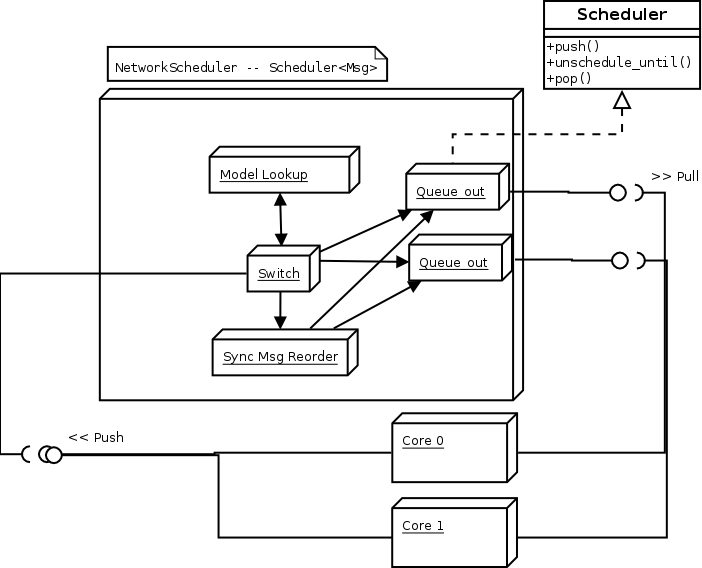
\includegraphics[width=\textwidth]{network.png}}
	\caption{Network cooperation diagram}
	\label{networkdesign}
\end{figure} 
Early benchmarks showed a repeatable throughput of 5e5 msg/s, with 4 kernels on modest hardware. The problems of (unintentional) out of order receipt and potential loss of messages are a non-issue in this context, since we use FIFO queues and loss of a message would implicate severe system failure (in which case message loss is the lesser problem).\\
Another advantage of hiding the message exchange behind a shared Network class instance is that, should this be required in the future, the kernel could run on different machines without requiring much redesigning of the system. An RPC implementation would simply have to implement the Network class on both sides.

\section{Tracing}
The tracing uses template programming, and is largely asynchronous w.r.t. the simulator kernels. This can be seen by the high utilization values when benchmarking the examples.
The tracing component makes heavy use of template programming. For more detailed information, please refer to \href{run:./tracersReport.pdf}{tracersReport.pdf}.

\section{Models}
The models hide all implementation details for the particular DEVS formalisms, without limiting the user to extend into any subclassed model of his/her choice. The use can focus on what he/she wants the model to emulate, and not worry about for example locking, allocation etc. We refer to the manual for more information about the creation of these models.

\section{Scheduler}
A Scheduler was implemented based on the prototyping code. As required, as list based scheduler was implemented. \\
The interface from PyPDevs' scheduler class was reused, but internally the scheduler class in our project differs on a few points. \\
\subsection{Composition}
All schedulers are based on a heap, which order items to be scheduled. We never actually schedule models, only entries (A struct containing name and time to schedule), allowing for far faster operation. This is complemented by a hashmap, so that entries can have O(1) lookup and erasure (required for the use case of antimessaging, among others). The operation massReschedule() was left out of the interface, since it can be easily composed using erase() and push\textunderscore back().
\\
\subsection{Implementation}
The actual heap used is either based on std::list as required, or one of Boost's heaps. The user is provided with a convenience factory function that creates Scheduler instances with varying heap backends. In general, the Fibonacci heap is one of the fastest, with skew heap sometimes coming out ahead. The list based heap is always a factor 2 slower, though again this depends on the usage scenario. \\Important to note is that only node based heaps can be used efficiently (without compromising the performance of erase() and contains()). We store on insertion an iterator with the key of the pushed element in the hashmap. This also works as a safety check, preventing double insertion (depending ofcourse on the hash-specialization semantics). This freedom of implementation is visible in the tracers where duplicate elements are allowed if they have a different address, contrasted with the model scheduler which disallows a model to be scheduled twice.\\
Finally, the std::hash$<>$ specialization used by the message scheduler allows O(1) annihilation of a message by its antimessage (since the hash is identical).
\subsection{Differences}
We intended to use the scheduler class not only for scheduling models, but also to store pending incoming messages, and tracing messages. To allow this, the Scheduler class only requires from a scheduled item that it has operator$<$ and std::hash$<$T$>$ defined.

\section{Controller}
For the controller, care was taken in making the interface both functional and minimal. The default configuration is quick to set up, and customization is possible should the user require it.

\section{Serialization}
For serialization we used the Cereal \cite{cereal} header-only framework. We opted for separate load and save functions for full flexibility. For each type that occurs in the form of a pointer we implemented a static load and construct method since the object first has to be created before the saved data can be imported. Cereal has a small coupling with the code (models) that has to be written by the user as the user has to register his own classes due to polymorphism.

All the main functionality to load objects is implemented in the serialize function itself. Most classes also have an implementation for load and construct so that objects can separately be constructed before filling it with the saved data. This is necessary in cases where pointers to objects of those classes have to be serialized or where there is no default constructor available. The implementation of those load and construct methods is always restricted to creating an object with - most of the time - meaningless temporary datamembers after which the serialize function of the created object is called to load the actual data.

Since Cygwin is not compatible with the std::to\_string() function, which is used for serialization to human readable formats like JSON or XML, only serialization to binary files is supported. Even in the binary archive implementation of Cereal the std::to\_string() function occurred, though only on non-decisive places, resulting in some slightly modified headers for this project.  The binary archives are lighter and give more speed than the user-readable formats but comes with the disadvantage of not providing full garanty that saved data can be correctly loaded on another architecture. 

Since Cereal was hard to use and gave a lot of undesired errors while serializing const datamembers and objects of purely virtual classes, we decided to violate some proper design rules to overcome this.

As we have experienced problems with an unressolved bug from Cereal - covering the errors in case of specific nested circular smart pointers - we were forced to not always follow the elegant design of Cereal and explicit force the calling of some serialization function in the load and construct functions.

\chapter{Non-functional requirements}
\section{Correctness}
\subsubsection{Testing}
The use of the jenkins CI was heavily leveraged, in combination with extensive testing. Any feature increment could only be merged into the project if it passed the developer's own jenkins instance.
\subsubsection{Thread races and deadlock}
Deadlocks and race conditions are very hard to debug, let alone prevent. To help us in this area as much as possible we used prototypes of threaded code in the tests before merging them into the main classes, and each build is checked with ThreadSanitizer \cite{tsan} which proved invaluable in preventing races and deadlocks in the threaded codepaths.
\subsubsection{Memory leaks and undefined behaviour}
With most entities represented as smart pointer, the need to ensure a leak free simulator nevertheless remained. To check for allocation misuse and a whole other series of errors we used Valgrind \cite{vg}. This meant for example that we detected a leak caused by circular referencing smart pointers.

\subsubsection{Teamwork}
We met at least once every week (barring the exam period), with each meeting having a formal report. Whenever required, teammembers used video conferencing to solve critical bugs or discuss design/coding issues.
\subsubsection{Code review}
Although there was no real formal code review done up to now, we've had several debug sessions reviewing each others code. This means the most critical used sections of the code are allready reasonably well reviewed, albeit not formally.
\subsubsection{Portability}
We develop on Unix, Windows and MacOSX.

In Windows we chose the Cygwin platform instead of MinGW to compile our project on. This because we make use of the C++11 std::thread objects; MinGW doesn't support POSIX threads. When building the project with GTest on Windows you need to use the -std=gnu++11 flag instead of the standard -std=c++11 flag, because we need the GNU extensions to correctly link everything.

\chapter{Functional requirements}
\section{DEVS Formalisms}
\subsection{Single core}
The single core implementations follow exactly the runtime behaviour shown by the PyPDEVS simulator. We've chosen to emulate the Select() function with an integer priority value the user can set. This saves 1 virtual function call per transition and can quite easily be optimized by the compiler since it remains constant.
\subsubsection{DirectConnect}
The directConnect algorithm has gone relatively unchanged from its implementation in PyPDEVS, though the role of the RootDEVS class has been simplified somewhat. Its main function has been reduced to executing directConnect and then storing the resulting list of connected atomic models.
\subsubsection{Dynamic Structured}
Dynamic structured DEVS is completely supported in single core simulation. This includes allowing the following structural changes during the simulation:
\begin{itemize}
	\item adding/removing connections
	\item adding/removing ports
	\item adding/removing submodels.
\end{itemize}
These changes are only allowed during a special phase of the simulation. The simulator provides a map object of type \lstinline[language=C++,basicstyle=\small\color{black}]{std::multimap<std::string, std::string>} that can be used for communication and cooperation between the models. During one simulation step, this communication always happens from bottom to top. Only models that had an internal transition are considered for performing dynamic structured.\\
Unlike the PyPDEVS, we will try to keep a removed model intact when it is removed from the simulation.
\subsection{Parallel}
\subsubsection{Optimistic}
Optimistic time synchronization requires an implementation of timewarp, and more extensive locking than would be required for conservative. The GVT algorithm (Mattern \cite{Mattern}) runs on a separate thread from the simulation kernel threads, so care must be taken that they don't deadlock, but don't race either.
\subsubsection{Conservative}
The implementation of the conservative formalism follows the algorithm as described in \cite{cons}. \\
\paragraph{Algorithm}
The following listing briefly states the steps required in the conservative synchronization algorithm.\\
Initialize eit,eot as (0,0) per kernel.\\
A Time object has an absolute first field , followed by a causal second field.\\
\begin{algorithm}
\caption{Conservative PDEVS}
\label{CHalgorithm}
\begin{algorithmic}
\Procedure{CPDEVS Modified}{}
\State 0.1 Construct a depency graph, determining which models influence this kernel directly
\State 0.2 If a msg is sent : eot = (timestamp > eot) ? timestamp : eot
\While{Termination trigger not reached}
\State 1. Simulate until vtime $>=$ eit
\State 1.a If msg is sent during sim : eot = max(timestamp, eot)
\State 2.a Time x = (eit + min lookahead, 0)
\State 2.b Time y = (msg sent) ? (eit,1) : (time next transition)
\State 2.c Time eot = std::min(x,y)
\State 2.d Share eot value with other kernels.
\State 3   Time eit = min ( $eot_i$ for i in influencing kernels)
\EndWhile
\EndProcedure
\end{algorithmic}
\end{algorithm}\\
\subparagraph{Differences with ADEVS}
A big difference between ADEVS' and our implementation is that we hold the eot-values of all kernels in shared memory. This means that step 1.a , which is normally done by the receiver when it inspects the message queue, can be done immediately. This also avoids the queueing delay incurred by simulation traffic.\\
Using the shared memory approach, we also avoid the sending of any synchronization message to other cores (required in ADEVS). \\In step 2.d we simply overwrite our old EOT value with the newly calculated. The shared EOT vector is only written at 1 position for each kernel , and only the influencing EOT values are ever read. \\
Also important to note is that there exist several edge cases not listed in this algorithm, but force the implementation to do more work than listed above. Consider a kernel with a non-dependent model A (that receives no input). By definition A has eit = oo, causing all eot-calculation to be skipped forever. We can't do this, if there exists at least 1 model depending on A, this model would get incorrect eot-values (either 0 or oo, which neither are correct since A is not prohibited from sending output).\\
The correct behaviour here is to replace eit with the vtime of the kernel at each simulation step and to use that in the algorithm.\\
 Furthermore, collecting lookahead values from models needs to be done in step 1, a lookahead value is calculated starting from the time it acquires a new state. This means that the lookahead value used in 2.a has to be continuously updated, regardless of usage, and has to be reset between simulation rounds (step 1 can entail several of such rounds). If we don't reset the minimum lookahead value in between rounds, there are scenarios where an incorrect minimum of a model that is no longer scheduled in the next round can warp the calculation. \\ 
 The calculation done in steps 2, 3 are quite efficiently implemented, although a future optimization could delay step 3 until several rounds have passed, more in line with the theoretical algorithm.
\subparagraph{Dependency calculation}
The author of the models needs to supply the kernel, for each model, with a list of models by whom it is influenced. Receiving a message that alters a model's output is defined as influencing in this context. Using the allocation information provided by the Controller, the Kernel will then determine which other Kernels (including possibly itself) it is dependent on.\\
It is important to note that the user need not interpret this dependency relation as transition, and needs to look only at 1-edge removed models. \\
To clarify this last point: suppose we have 3 models A, B, C with A sending output to B, and B to C. C is indirectly influenced by A, but need not record this information (which is non trivial to retrieve for a non-trivial model, disregarding cycles for the moment). \\
Let A be allocated @ kernel 0, B @ 1, C @ 2. While the dependency is transitive, since kernel 1 is already bound by kernel 0, kernel 2 does not require kernel 0's information (eot). By moving this transitivity to the kernel level, the model's author only has to look at 1-edge distant dependencies. \\
At construction a Conservative Kernel will collect , for each model it holds, the list of names of influencing models. Next, the kernel requests for each unique name the allocation information (O(1) lookup). Note that this can be optimized if the model stores its allocation information, but this then prohibits runtime reallocation should this be implemented in the future.

\chapter{Obstacles}
\section{Virtualization}
Virtualization proved a significant hurdle by exposing potential faults. Standard compliant code was found to be leaking memory by not calling container member destructors but only on a VM with Linux as Guest and Windows as Host. This was never reproducible in another setting.
\section{Threading}
\subsection{String}
libstdc++'s std::string implementation appears to be still Copy On Write (despite 21.4.1 p6 from the C++ standard) \cite{cpp}. This triggers an alert by threadsanitizer for a possible race whenever a string was supposedly copied but internally still stored as a reference to the same object. Explicitly invoking the string constructor with the char[] of the original string, proved to be a safe workaround here. Note that this problem is a known issue \cite{cow}, which is solved in GCC 5.1.\\
\subsection{Timing}
We also encountered several scenarios where thread scheduling complicated our kernel control code. An extreme example of this is Valgrind, which can cause multithreaded code to be executed sequentially. This can be fatal for a parallel simulator if a dependent core is scheduled before the influencing core is ever executed. Modifying valgrind's invocation can alleviate this, but there remain edge cases where a core/kernel can get into a state where it can no longer advance (depending on the model composition). The simulator detects this and (eventually) halts the simulation. \\ Note that the above problem is not limited to valgrind, on Virtualized system this is more easily triggered than in a non virtualized setting.\\
Furthermore, we also force an idle kernel (a kernel that has either reaches termination time, or can't advance time (no messages and no scheduled models) to yield/sleep for a short duration. The reason for this behaviour is to allow the other cores execution time, which would otherwise be spent in idling loops. A condition variable was evaluated as a solution, but not implemented since it also suffered from timing issues (time between thread awakening and core simulating).
\section{Heaps}
2 of the Heaps we use in the Scheduler proved to have subtle corrupting bugs, which were only found quite late in the project. Boost's binomial heap, for reasons so far unknown, sometimes fails to deallocate/remove nodes/items. The actual failure is masked until the next insertion, where we then triggered one of our own invariant checks (the heap size was no longer equal to that of the hashmap). It should be noted that we already experienced similar issues with the binomial heap not deallocating memory despite size() returning 0. \\ Time prevented us from writing up a formal bug report, since the bug is hard to reproduce and even harder to detect.
The D-ary heap triggered an move-assing to self assertion when we used the Debugging version of the STL, so we had to remove both from our Schedulers. This is no way impacted performance, as the Fibonacci heap was in practice faster (with the skew heap sometimes overtaking it).
\section{Toolchains}
To develop we used the required toolchains:\\ g++/clang++ as compiler, Eclipse+CDT as IDE, git for dvcs, jenkins as ci, cmake as build tool supplemented with some shell and python scripting.
The plot plugin from Jenkins was used to do perfomance regression testing, but the plugin itself is not that stable. Nonetheless, we detected several random regression using the plotted graphs. \\
G++ failed with an internal compiler error in certain multi-build cmake scenario's, for which a  bug was filed \cite{gpp}. GDB also intermittently failed with a segmentation fault when debugging threaded code. Using Fedora's bug reporting mechanism abrt a bug \cite{gdb} was filed for this as well.
\section{Logger}
The recommended logger (g3log), while powerful and fast, proved a dead end since it does not compile on Cygwin. 
Stijn therefore wrote his own implementation.\\
This implementation only covers the most basic needs:
\begin{itemize}
	\item asynchronous output
	\item thread safe
	\item multiple logging levels currently, the following 4 levels are supported:\\
		\emph{INFO}, \emph{DEBUG}, \emph{WARNING} and \emph{ERROR}
	\item levels can be individually switched on/off at compile time
	\item No logging code is executed whatsoever if the logger is disabled.
	\item log messages contain file name and line number of the log command.
	\item basic crash safety. The logger will catch the following signals and flush all remaining output before exiting the program:
		\begin{itemize}
			\item \emph{SIGSEGV} Segmentation fault, sent by the operating system.
			\item \emph{SIGTERM} Termination request, sent by the program.
			\item \emph{SIGABRT} Abort --- abnormal termination, e.g. when an assertion fails.
			\item \emph{SIGINT} Interrupt, used for catching crtl+C, which is useful for debugging deadlocks.
		\end{itemize}
\end{itemize}

\paragraph{Asynchronous output}
To implement the asynchronous output, we made use of a custom stream buffer. The original design is by Dietmar K{\"u}hl \cite{asynchwrite}. We modified this design in order to make it thread safe.

\section{Jenkins}
While building the traffic system on the Jenkins server problems occured and the server crashed due to a memory shortage. A lower level of optimization solved this problem.

\chapter{Performance analysis}
To measure the performance of \textsc{DEVS Ex Machina} under more demanding conditions, \textbf{DEVStone} and \textbf{PHOLD} benchmarks were used in combination with the \texttt{perf} profiler tool. As these are standardized tests, they allow easy comparison between our implementation and \textit{PythonPDEVS}.\\
\\
{\footnotesize[All the following tests were performed using an \textit{Intel Core i5 M520} CPU at 2.40GHz, parallel testing was done using 2 simulation cores unless mentioned otherwise. Compilation was done with the \texttt{-O3} optimization flag. All tests were ran 5 times to give an indication of the predictability of the result.]}

\pagebreak

\section{DEVStone}
\begin{figure}
\centering
\begin{minipage}{.5\textwidth}
  \centering
  \hspace*{-1.5in}
  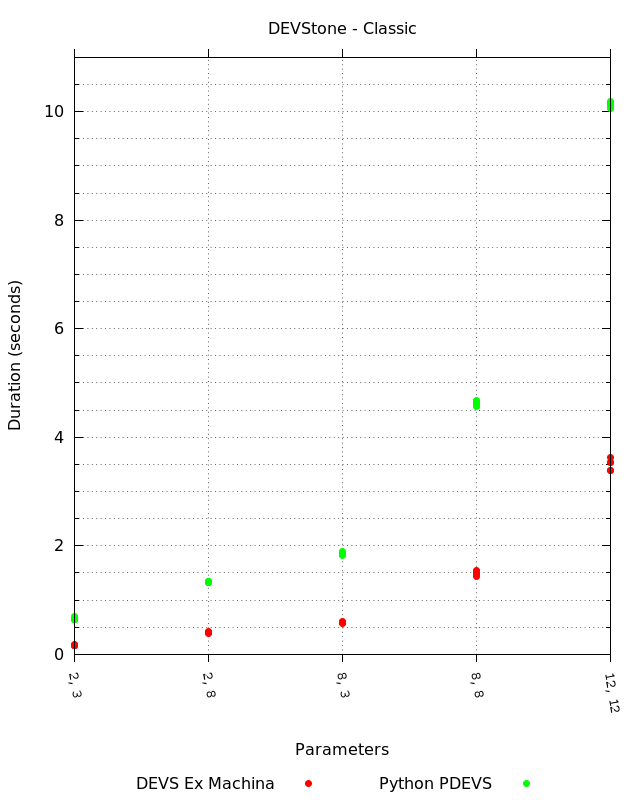
\includegraphics[width=1.6\linewidth]{devstone_classic.png}
\end{minipage}%
\begin{minipage}{.5\textwidth}
  \centering
  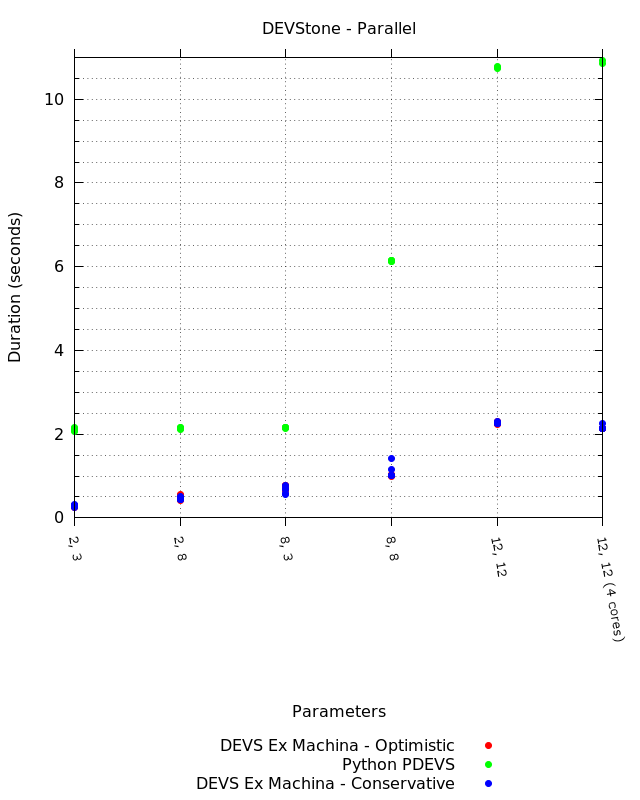
\includegraphics[width=1.6\linewidth]{devstone_parallel.png}
\end{minipage}
\end{figure}

In both Classic and Parallel DEVS there are noticeable speedups compared to \textit{PyPDEVS}.\\
Looking at \textsc{DEVS Ex Machina} specifically we can see that in the first few, rather lightweight cases the single core Classic DEVS simulation is faster than PDEVS, in the first case even twice as fast. Once more models start to get involved however, things quickly turn around since the benefit of having the raw processing power of more cores available outweighs the cost of setting up and managing multiple threads.\\
Additionally, the final and most demanding test case, a DEVStone benchmark of depth and width 12, was also executed with 4 cores, which showed a slight improvement over using 2 cores.
\\

However, it should be noted that in PDEVS a somewhat thought-out assignment of models to cores is of critical importance. A parallel simulation with models placed haphazardly can perform \emph{significantly} worse than a Classic DEVS which doesn't have to deal with placement. In general, it is best to keep the most used connections intra-core.

\pagebreak

\section{PHOLD}
\begin{figure}
\centering
\begin{minipage}{.5\textwidth}
  \centering
  \hspace*{-1.5in}
  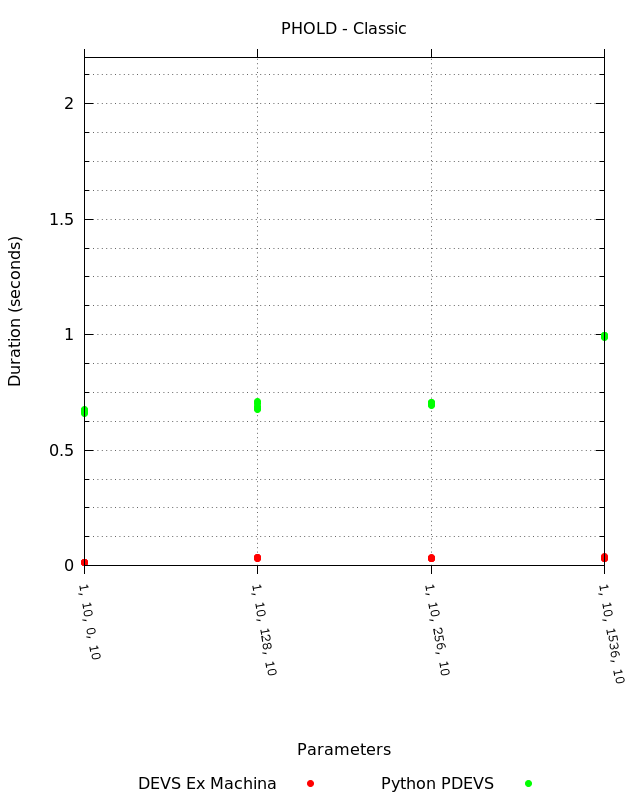
\includegraphics[width=1.6\linewidth]{phold_classic.png}
\end{minipage}%
\begin{minipage}{.5\textwidth}
  \centering
  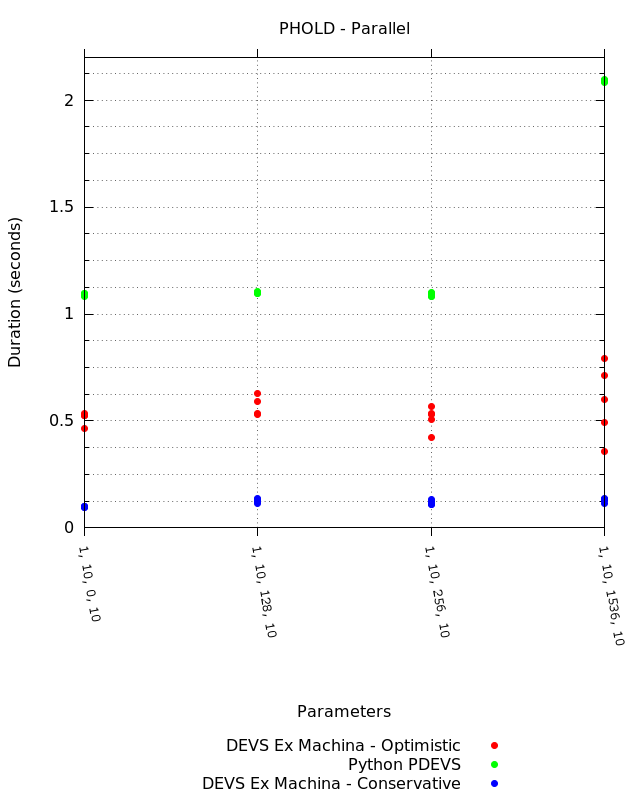
\includegraphics[width=1.6\linewidth]{phold_parallel.png}
\end{minipage}
\end{figure}

{\footnotesize[ To make a useful comparison with \textit{Python PDEVS} possible, care was taken to make sure the "meaningless" computations related to the payload size were not removed by compiler optimisations ]}\\
\\
This benchmark tests the effect of different payload sizes in a highly interconnected environment.\\
In both environments \textsc{DEVS Ex Machina} is significantly faster than \textit{PyPDEVS}.
Especially interesting is the second graph with parellel results. Whereas in DEVStone Optimistic and Conservative DEVS performed relatively equally, here we can spot a clear discrepancy between them.

In Optimistic we can see that as the payload grows, the total runtime becomes less predictable. Because of the inherent interconnectivity of the benchmark (lots of inter-core communication), and because processing a message with a larger payload can take a while, the chance of reverts or even series of reverts is increased.

In Conservative simulation however, the flow time is tightly controlled, avoiding reverts. In this case this behavior leads to significantly better results.

\pagebreak

\section{Detailed stats}
Some more detailed statistics provided by \texttt{perf} are shown here. Each time, only the result of a single run is provided, to give a general indication.

\subsection{DEVStone}
\paragraph{\textsc{DEVS Ex Machina}}
\begin{Verbatim}[fontsize=\small]
$ perf stat ./dxexmachina_devstone classic 2 3
 Performance counter stats for './dxexmachina_devstone classic 2 3':

        189.176880 task-clock (msec)         #    1.115 CPUs utilized          
               243 context-switches          #    0.001 M/sec                  
               212 cpu-migrations            #    0.001 M/sec                  
               691 page-faults               #    0.004 M/sec                  
       476,733,288 cycles                    #    2.520 GHz                     [84.35%]
       204,107,284 stalled-cycles-frontend   #   42.81% frontend cycles idle    [84.40%]
        95,948,277 stalled-cycles-backend    #   20.13% backend  cycles idle    [67.48%]
       561,945,984 instructions              #    1.18  insns per cycle        
                                             #    0.36  stalled cycles per insn [85.07%]
       132,785,648 branches                  #  701.913 M/sec                   [84.93%]
         1,847,286 branch-misses             #    1.39% of all branches         [84.62%]

       0.169685736 seconds time elapsed
       
$ perf stat ./dxexmachina_devstone opdevs 2 2 3
 Performance counter stats for './dxexmachina_devstone opdevs 2 2 3':

        258.435415 task-clock (msec)         #    0.924 CPUs utilized          
             1,201 context-switches          #    0.005 M/sec                  
                26 cpu-migrations            #    0.101 K/sec                  
             3,836 page-faults               #    0.015 M/sec                  
       613,419,141 cycles                    #    2.374 GHz                     [83.93%]
       316,632,123 stalled-cycles-frontend   #   51.62% frontend cycles idle    [85.01%]
       139,998,026 stalled-cycles-backend    #   22.82% backend  cycles idle    [67.52%]
       615,911,601 instructions              #    1.00  insns per cycle        
                                             #    0.51  stalled cycles per insn [84.95%]
       144,090,841 branches                  #  557.551 M/sec                   [85.11%]
         2,820,791 branch-misses             #    1.96% of all branches         [78.96%]

       0.279720722 seconds time elapsed

$ perf stat ./dxexmachina_devstone cpdevs 2 2 3
 Performance counter stats for './dxexmachina_devstone cpdevs 2 2 3':

        257.663639 task-clock (msec)         #    0.851 CPUs utilized          
               911 context-switches          #    0.004 M/sec                  
                19 cpu-migrations            #    0.074 K/sec                  
             3,837 page-faults               #    0.015 M/sec                  
       663,670,571 cycles                    #    2.576 GHz                     [82.64%]
       351,293,037 stalled-cycles-frontend   #   52.93% frontend cycles idle    [82.43%]
       197,270,653 stalled-cycles-backend    #   29.72% backend  cycles idle    [65.25%]
       643,477,063 instructions              #    0.97  insns per cycle        
                                             #    0.55  stalled cycles per insn [84.74%]
       150,533,837 branches                  #  584.226 M/sec                   [87.77%]
         2,968,904 branch-misses             #    1.97% of all branches         [82.67%]

       0.302693494 seconds time elapsed
\end{Verbatim}
\paragraph{\textsc{PythonPDEVS}}
\begin{Verbatim}[fontsize=\small]
$ perf stat ./dxexmachina_devstone classic 2 3
 Performance counter stats for 'python ./DEVStone/experiment.py default 2 false':

        670.501187 task-clock (msec)         #    0.959 CPUs utilized          
               169 context-switches          #    0.252 K/sec                  
                22 cpu-migrations            #    0.033 K/sec                  
             4,962 page-faults               #    0.007 M/sec                  
     1,828,074,336 cycles                    #    2.726 GHz                     [82.96%]
       983,729,421 stalled-cycles-frontend   #   53.81% frontend cycles idle    [83.51%]
       600,902,567 stalled-cycles-backend    #   32.87% backend  cycles idle    [67.59%]
     1,691,525,594 instructions              #    0.93  insns per cycle        
                                             #    0.58  stalled cycles per insn [84.05%]
       380,934,259 branches                  #  568.134 M/sec                   [83.42%]
        15,797,482 branch-misses             #    4.15% of all branches         [82.57%]

       0.699383675 seconds time elapsed
       
$ perf stat ./dxexmachina_devstone opdevs 2 2 3
 Performance counter stats for 'mpirun -np 2 python ./DEVStone/experiment.py default 2 false':

        692.210888 task-clock (msec)         #    0.330 CPUs utilized          
               909 context-switches          #    0.001 M/sec                  
                99 cpu-migrations            #    0.143 K/sec                  
             8,728 page-faults               #    0.013 M/sec                  
     1,801,930,537 cycles                    #    2.603 GHz                     [82.89%]
       929,771,707 stalled-cycles-frontend   #   51.60% frontend cycles idle    [82.88%]
       581,151,775 stalled-cycles-backend    #   32.25% backend  cycles idle    [68.37%]
     1,800,262,136 instructions              #    1.00  insns per cycle        
                                             #    0.52  stalled cycles per insn [84.52%]
       403,185,223 branches                  #  582.460 M/sec                   [84.04%]
        13,159,671 branch-misses             #    3.26% of all branches         [82.92%]

       2.099629915 seconds time elapsed
\end{Verbatim}
\subsection{PHOLD}
\paragraph{\textsc{DEVS Ex Machina}}
\begin{Verbatim}[fontsize=\small]
$ perf stat ./dxexmachina_phold classic 1 10 0 10
 Performance counter stats for './dxexmachina_phold classic 1 10 0 10':

         12.815382 task-clock (msec)         #    1.081 CPUs utilized          
                11 context-switches          #    0.858 K/sec                  
                25 cpu-migrations            #    0.002 M/sec                  
               712 page-faults               #    0.056 M/sec                  
        27,657,920 cycles                    #    2.158 GHz                     [64.22%]
        13,070,687 stalled-cycles-frontend   #   47.26% frontend cycles idle    [75.41%]
         8,563,853 stalled-cycles-backend    #   30.96% backend  cycles idle   
        31,010,010 instructions              #    1.12  insns per cycle        
                                             #    0.42  stalled cycles per insn
         6,957,728 branches                  #  542.920 M/sec                  
           122,049 branch-misses             #    1.75% of all branches         [69.03%]

       0.011857863 seconds time elapsed
       
$ perf stat ./dxexmachina_phold opdevs 2 1 10 0 10
 Performance counter stats for './dxexmachina_phold opdevs 2 1 10 0 10':

         58.345592 task-clock (msec)         #    0.103 CPUs utilized          
               235 context-switches          #    0.004 M/sec                  
                24 cpu-migrations            #    0.411 K/sec                  
               844 page-faults               #    0.014 M/sec                  
        86,073,977 cycles                    #    1.475 GHz                     [79.15%]
        41,603,661 stalled-cycles-frontend   #   48.33% frontend cycles idle    [87.74%]
        23,030,593 stalled-cycles-backend    #   26.76% backend  cycles idle    [54.61%]
        93,532,407 instructions              #    1.09  insns per cycle        
                                             #    0.44  stalled cycles per insn [79.51%]
        20,525,076 branches                  #  351.785 M/sec                   [88.38%]
           426,419 branch-misses             #    2.08% of all branches         [93.36%]

       0.564278040 seconds time elapsed
       
$ perf stat ./dxexmachina_phold cpdevs 2 1 10 0 10
 Performance counter stats for './dxexmachina_phold cpdevs 2 1 10 0 10':

         45.097489 task-clock (msec)         #    0.453 CPUs utilized          
                46 context-switches          #    0.001 M/sec                  
                13 cpu-migrations            #    0.288 K/sec                  
               856 page-faults               #    0.019 M/sec                  
        68,793,923 cycles                    #    1.525 GHz                     [67.00%]
        40,973,357 stalled-cycles-frontend   #   59.56% frontend cycles idle    [82.61%]
        15,619,202 stalled-cycles-backend    #   22.70% backend  cycles idle    [71.88%]
        56,478,836 instructions              #    0.82  insns per cycle        
                                             #    0.73  stalled cycles per insn [91.10%]
        13,722,715 branches                  #  304.290 M/sec                   [91.32%]
           279,636 branch-misses             #    2.04% of all branches         [90.09%]

       0.099622680 seconds time elapsed
\end{Verbatim}
\paragraph{\textsc{PythonPDEVS}}
\begin{Verbatim}[fontsize=\small]
$ perf stat ./dxexmachina_phold classic 1 10 0 10
 Performance counter stats for 'python ./benchmarks/experiment.py':

        671.561546 task-clock (msec)         #    0.998 CPUs utilized          
                97 context-switches          #    0.144 K/sec                  
                18 cpu-migrations            #    0.027 K/sec                  
             2,974 page-faults               #    0.004 M/sec                  
     1,916,305,122 cycles                    #    2.854 GHz                     [83.35%]
     1,005,734,716 stalled-cycles-frontend   #   52.48% frontend cycles idle    [83.34%]
       499,103,479 stalled-cycles-backend    #   26.05% backend  cycles idle    [66.69%]
     2,060,775,055 instructions              #    1.08  insns per cycle        
                                             #    0.49  stalled cycles per insn [83.34%]
       345,264,964 branches                  #  514.123 M/sec                   [83.89%]
        12,293,319 branch-misses             #    3.56% of all branches         [82.87%]

       0.673223302 seconds time elapsed
       
$ perf stat ./dxexmachina_phold opdevs 2 1 10 0 10
 Performance counter stats for 'mpirun -np 2 python ./benchmarks/experiment.py':

        866.680461 task-clock (msec)         #    0.800 CPUs utilized          
               929 context-switches          #    0.001 M/sec                  
                83 cpu-migrations            #    0.096 K/sec                  
             7,466 page-faults               #    0.009 M/sec                  
     2,326,077,914 cycles                    #    2.684 GHz                     [83.64%]
     1,283,069,850 stalled-cycles-frontend   #   55.16% frontend cycles idle    [83.95%]
       940,158,530 stalled-cycles-backend    #   40.42% backend  cycles idle    [65.55%]
     2,325,361,346 instructions              #    1.00  insns per cycle        
                                             #    0.55  stalled cycles per insn [82.69%]
       402,983,176 branches                  #  464.973 M/sec                   [83.67%]
        15,476,432 branch-misses             #    3.84% of all branches         [84.05%]

       1.083881333 seconds time elapsed
\end{Verbatim}

\section{Compared to \textsc{ADEVS}}
Since the DEVStone benchmark for \textsc{ADEVS} does not support different depths, a test with greater width was performed instead. As we can see, \textsc{ADEVS} is still quite a bit faster.
\paragraph{\textsc{DEVS Ex Machina} - Classic DEVS}
\begin{Verbatim}[fontsize=\small]
$ perf stat ./dxexmachina_devstone classic 32 0

 Performance counter stats for './dxexmachina_devstone classic 32 0':

        800.259000 task-clock (msec)         #    1.081 CPUs utilized          
             2,178 context-switches          #    0.003 M/sec                  
               217 cpu-migrations            #    0.271 K/sec                  
               767 page-faults               #    0.958 K/sec                  
     2,199,059,849 cycles                    #    2.748 GHz                     [83.12%]
       862,325,341 stalled-cycles-frontend   #   39.21% frontend cycles idle    [83.36%]
       432,658,584 stalled-cycles-backend    #   19.67% backend  cycles idle    [67.64%]
     2,794,549,736 instructions              #    1.27  insns per cycle        
                                             #    0.31  stalled cycles per insn [84.75%]
       661,425,743 branches                  #  826.515 M/sec                   [84.04%]
         9,605,392 branch-misses             #    1.45% of all branches         [82.83%]

       0.739954252 seconds time elapsed
\end{Verbatim}
\paragraph{\textsc{ADEVS} - Classic DEVS}
\begin{Verbatim}[fontsize=\small]
$ perf stat ./sim 32 0

 Performance counter stats for './sim 32 0':

         15.465233 task-clock (msec)         #    0.976 CPUs utilized          
                 1 context-switches          #    0.065 K/sec                  
                 1 cpu-migrations            #    0.065 K/sec                  
               340 page-faults               #    0.022 M/sec                  
        22,395,954 cycles                    #    1.448 GHz                     [74.20%]
         6,618,757 stalled-cycles-frontend   #   29.55% frontend cycles idle    [74.17%]
         2,895,009 stalled-cycles-backend    #   12.93% backend  cycles idle    [87.88%]
        31,797,999 instructions              #    1.42  insns per cycle        
                                             #    0.21  stalled cycles per insn
         6,645,494 branches                  #  429.705 M/sec                  
           250,467 branch-misses             #    3.77% of all branches         [74.03%]

       0.015852985 seconds time elapsed
\end{Verbatim}

\section{Compared to PyPDEVS on PyPy}
Surprisingly, both DEVStone and PHOLD perform significantly worse using \textit{PyPy} instead of \textit{CPython}, despite the sometimes dramatically improved CPU utilization. Perhaps these two test cases just happen to be "JIT-unfriendly".\\
\textit{PyPy} is known to sometimes perform worse when profiling but informally its speed didn't seem any different when running the benchmarks without using \texttt{perf}.

\subsection{DEVStone}
\paragraph{\textsc{PythonPDEVS} - Classic DEVS on PyPy}
\begin{Verbatim}[fontsize=\small]
$ perf stat pypy experiment.py default 3 false > out.txt

 Performance counter stats for 'pypy experiment.py default 3 false':

       2367.165094 task-clock (msec)         #    0.998 CPUs utilized          
               276 context-switches          #    0.117 K/sec                  
                20 cpu-migrations            #    0.008 K/sec                  
            11,357 page-faults               #    0.005 M/sec                  
     6,765,226,427 cycles                    #    2.858 GHz                     [83.37%]
     4,234,478,457 stalled-cycles-frontend   #   62.59% frontend cycles idle    [83.27%]
     3,145,973,412 stalled-cycles-backend    #   46.50% backend  cycles idle    [66.67%]
     5,014,442,675 instructions              #    0.74  insns per cycle        
                                             #    0.84  stalled cycles per insn [83.49%]
     1,077,122,966 branches                  #  455.027 M/sec                   [83.44%]
        38,104,090 branch-misses             #    3.54% of all branches         [83.27%]

       2.372239526 seconds time elapsed
\end{Verbatim}
\paragraph{\textsc{PythonPDEVS} - Parallel DEVS on PyPy}
\begin{Verbatim}[fontsize=\small]
$ perf stat mpirun -np 2 pypy experiment.py default 3 false > out.txt

 Performance counter stats for 'mpirun -np 2 pypy experiment.py default 3 false':

       5789.446884 task-clock (msec)         #    1.991 CPUs utilized          
               624 context-switches          #    0.108 K/sec                  
                40 cpu-migrations            #    0.007 K/sec                  
            23,245 page-faults               #    0.004 M/sec                  
    15,328,712,962 cycles                    #    2.648 GHz                     [83.32%]
    10,258,365,662 stalled-cycles-frontend   #   66.92% frontend cycles idle    [83.32%]
     7,799,638,758 stalled-cycles-backend    #   50.88% backend  cycles idle    [66.54%]
    10,156,225,688 instructions              #    0.66  insns per cycle        
                                             #    1.01  stalled cycles per insn [83.23%]
     2,163,097,214 branches                  #  373.628 M/sec                   [83.47%]
        76,428,341 branch-misses             #    3.53% of all branches         [83.42%]

       2.907224325 seconds time elapsed
\end{Verbatim}
\subsection{PHOLD}
\paragraph{\textsc{PythonPDEVS} - Classic DEVS on PyPy}
\begin{Verbatim}[fontsize=\small]
$ perf stat pypy experiment.py > out.txt

 Performance counter stats for 'pypy experiment.py':

       1827.849910 task-clock (msec)         #    0.999 CPUs utilized          
               220 context-switches          #    0.120 K/sec                  
                10 cpu-migrations            #    0.005 K/sec                  
            14,385 page-faults               #    0.008 M/sec                  
     5,224,512,160 cycles                    #    2.858 GHz                     [83.37%]
     3,283,008,184 stalled-cycles-frontend   #   62.84% frontend cycles idle    [83.37%]
     2,563,366,886 stalled-cycles-backend    #   49.06% backend  cycles idle    [66.80%]
     4,079,915,131 instructions              #    0.78  insns per cycle        
                                             #    0.80  stalled cycles per insn [83.42%]
       758,611,592 branches                  #  415.029 M/sec                   [83.37%]
        28,841,978 branch-misses             #    3.80% of all branches         [83.16%]

       1.830573045 seconds time elapsed
\end{Verbatim}
\paragraph{\textsc{PythonPDEVS} - Parallel DEVS on PyPy}
\begin{Verbatim}[fontsize=\small]
$ perf stat mpirun -np 2 pypy experiment.py > out.txt

 Performance counter stats for 'mpirun -np 2 pypy experiment.py':

       5410.417506 task-clock (msec)         #    1.992 CPUs utilized          
               785 context-switches          #    0.145 K/sec                  
                33 cpu-migrations            #    0.006 K/sec                  
            28,874 page-faults               #    0.005 M/sec                  
    15,456,764,898 cycles                    #    2.857 GHz                     [83.35%]
    12,040,987,764 stalled-cycles-frontend   #   77.90% frontend cycles idle    [83.35%]
     6,550,209,612 stalled-cycles-backend    #   42.38% backend  cycles idle    [66.70%]
     7,709,537,731 instructions              #    0.50  insns per cycle        
                                             #    1.56  stalled cycles per insn [83.41%]
     1,430,492,329 branches                  #  264.396 M/sec                   [83.42%]
        63,358,010 branch-misses             #    4.43% of all branches         [83.21%]

       2.716329957 seconds time elapsed
\end{Verbatim}

\section{Logger}
We have also conducted a small benchmark to compare the raw power of our logger and the proposed g3log.
We let each logger print several hundred thousand messages to a file. These are the performance statistics:
\subsubsection{g3log}
\lstinputlisting[]{g3log.perf}
\subsubsection{Our own logger}
\lstinputlisting[]{own.perf}
\subsubsection{Conclusion}
While the difference is considerable, we should keep in mind that g3log generates timestamps for each message. It also contains several features that our logger doesn't, such as a more extensive crash safety. Moreover, g3log allows the user to dynamically change which log levels are filtered, while this can only be decided at compile time for our logger. This can be clearly seen in the amount of branches taken by the program.

\chapter{Examples}
As part of the assignment we've implemented a set of examples for our simulator. Most of them are based on models already described in Yentl's thesis. 

\subsubsection{Traffic light and Traffic System}
These simple models are an exact copy of those used as examples in pypdevs.

\subsubsection{DEVStone}
DEVStone is a standardized benchmark for DEVS. It can be run using the separate executable \texttt{dxexmachina\_devstone}. If this executable has not been generated, run the following command from the \texttt{build} folder: \texttt{make dxexmachina\_devstone}\\
The executable takes a few arguments. First you can specify whether you want to run it in Classic DEVS mode (\texttt{classic}) or Parallel (\texttt{opdevs} and \texttt{cpdevs} for Optimistic and Conservative respectively) followed by the amount of cores.\\
Next you can specify the width and the depth of the benchmark. By default this is 2 and 3.

\subsubsection{PHOLD}
PHOLD simulates a highly interconnected environment. Running it follows a procedure largely similar to \textbf{DEVStone}. The benchmark runs from a separate executable \texttt{dxexmachina\_phold}.\\
Again, its first arguments are the type of simulation. What follows is, in order, the amount of nodes in the \textbf{PHOLD}, the amount of atomic models per node, the size of the payload, and the percentage of remotes.

\subsubsection{Forestfire}
...\\
\\
\textbf{NOTE} We added an extra executable to the project containing only the necessary implementation for the traffic system model to work.

\subsubsection{Traffic system}
The \textbf{traffic system} is based on the traffic system described in Yentl's paper. We've implemented two versions, a bigger one and a smaller one.\\
A modified version of Yenl's script generates the header and source file for the city model and makes it possible to easily adopt the models size. The script can be found in the './main/script' folder of our repository.\\
\\
Run the following command to generate a city:
\begin{Verbatim}[fontsize=\small]
$ python script_devsexmachina.py {x} {y} {nodes} {districts}
\end{Verbatim}
The small city is 10 x 50 segments large and the larger city exists of 10 x 500 segments. Both cities are generated for 50 nodes and 5 districts as described in Yentl's thesis.\\
\\
\textbf{NOTE} We added an extra executable to the project containing only the necessary implementation for the traffic system model to work. This executable contains the larger version of the city. To build large cities you have to ensure that there is a sufficient amount of memory available. 

\subsubsection{Virus}
\begin{wrapfigure}{r}{0.3\textwidth}
  \begin{center}
    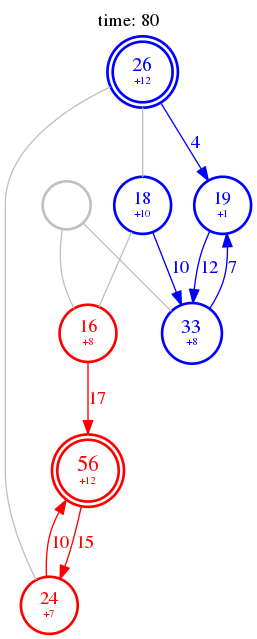
\includegraphics[width=0.28\textwidth]{virus}
  \end{center}
\end{wrapfigure}

Virus simulates the spread of two viruses over a pool of healthy cells.\\

The procedure is quite simple: each type of virus starts out in a single cell. Every cell, once in control of a virus, produces a set number of new viruses every turn and also sends out some of its contained viruses to a neighbour; this can be a neutral cell (thereby taking it over), a friendly cell (reenforcing it) or a cell owned by the other virus (reducing its numbers and possibly taking over the cell).\\
As a result this produces quite dynamic behavior, with both viruses spreading and moving around the pool or getting into stalemates.\\

This model is relatively interesting because it is well-connected and gradually produces more and more messages. Just like \textbf{PHOLD} it has performance gains in Conservative PDEVS over Optimistic.\\
\\
\textbf{Virus} has its own separate executable, \texttt{dxexmachina\_virus} which can be generated and used just like those of \textbf{DEVStone} and \textbf{PHOLD}. After specifying the simulation type the arguments are respectively the size of the cell pool (apart from the two starting cells), and the maximum amount of connections per cell.


\begin{thebibliography}{1}


  \bibitem{cow} \url{https://gcc.gnu.org/bugzilla/show_bug.cgi?id=21334#c47}

  \bibitem{Mattern} \url{http://citeseerx.ist.psu.edu/viewdoc/summary?doi=10.1.1.111.2811}
  
  \bibitem{gil} \url{https://wiki.python.org/moin/GlobalInterpreterLock}
  
  \bibitem{tsan} \url{https://code.google.com/p/thread-sanitizer/}
  
  \bibitem{vg} \url{http://valgrind.org/}
  
  \bibitem{perf} \url{https://perf.wiki.kernel.org/index.php/Main_Page}
  
  \bibitem{cereal} \url{https://uscilab.github.io/cereal/}
  
  \bibitem{cpp} \url{http://www.open-std.org/jtc1/sc22/wg21/docs/papers/2014/n4296.pdf}
  
  \bibitem{cons}  J. J. Nutaro, Building Software for Simulation: Theory and Algorithms, with
Applications in C++. Wiley Publishing, 2010.

  \bibitem{gpp}  \url{https://bugzilla.redhat.com/show_bug.cgi?id=1219175}
  
  \bibitem{gdb}  \url{https://bugzilla.redhat.com/show_bug.cgi?id=1219180}

  \bibitem{asynchwrite} \url{http://stackoverflow.com/a/21127776}

  \end{thebibliography}
\end{document}
